\documentclass[10pt,a4paper,hidelinks]{article}
\usepackage{lipsum}
\usepackage{url}
\usepackage{graphicx}
\usepackage[nochapters]{classicthesis} % nochapters

\begin{document}
    \pagestyle{plain}
    \title{\rmfamily\normalfont\spacedallcaps{Improving Wastewater treatment}}
    \author{\spacedlowsmallcaps{Eko J. Salim \& Gerraldo S. Candra}}
    \date{} % no date
    
    \maketitle
    
    \begin{abstract}
        \noindent Current wastewater treatment processes and technologies left much to be desired. Wastewater could be a valuable source of energy --- about 9 times more energy are in wastewater compared to the energy needed to proccess them in a modern plant. Present processes do not generally take this into account moreover, they are also generally inefficient and 'unclean'. Combining present technologies, such as and especially Microbial Fuel Cell (MFC) could help alleviate these present issues considering wastewater treatment. 
    \end{abstract}
       
    \tableofcontents
    
    \section{Processes}
    Various technologies are available for wastewater treatment: from activated sludges to vacuum evaporation. Combining these technologies below could lead into a sustainable wastewater treatment.
    \subsection{Microbial Fuel Cell}
    Microbial fuel cells are devices that drives a current using bacterias. Bacterias in a microbial fuel cell serve as catalyst to oxidize both organic
and inorganic matters.  The electrons from this oxidation are transferred to the anode and then to the cathode.  The 'how' electrons are transferred to anode serves as the distinction between two general types of MFC. In mediator microbial fuel cell, there exists a redox mediator which ‘shuttles’ electrons to the anode. A microbial fuel cell is classified as a mediator-less MFC if no exogenous mediators are added,  the method ofelectrons transfer in these instances can be by the following: direct membrane associated electron transfer, bacteria’s ‘nanowires’ . . .


In most MFCs, the electrons that reach the cathode combine with protons
that diffuse from the anode and oxygen provided from the  air;  the  resulting  product  is  water.   Chemical  oxidizers  may  also  be
used however because they need to replaced, they are not practical outisde laboratory use.

As MFCs break down organic matters and produce electricity, MFCs have found a use in wastewater treatment.

	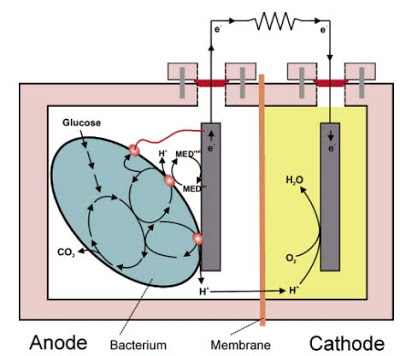
\includegraphics[scale=0.75]{gfx/mfc}
    \subsection{Anaerobic Digestion}
    \subsection{Algae}
    \subsection{Membrane Seperation}
    \subsection{Struvite Precipitation}
    \section{A Section}
    \lipsum[1]
    
    % Bibliography
    \nocite{*}
    \addtocontents{toc}{\protect\vspace{\beforebibskip}}
    \addcontentsline{toc}{section}{\refname}    
    \bibliographystyle{plain}
    \bibliography{Bibliography}
\end{document}